\chapter{Implementierung}


%\begin{itemize}
%  \item \textbf{Anforderungen} Welche Anforderungen muss der Prototyp erfüllen?
%  \item \textbf{Umsetzung} Architektur und Implementierung des Prototypen.
%  \item \textbf{Einbindung in OSSIM} An welcher Stelle wird er in das SIEM-System integriert? Abwägung der verschiedenen Möglichkeiten.
%  \item \textbf{Umsetzung des Schwellwertschemas} Implementierung des Schwellwertschemas und Integration in den Prototypen. Hier auch Key Management.
%\end{itemize}

\todo{Einführender Absatz}

\label{cha_implementation}



\section{Anforderungen}

\label{sec_impl_requirements}

Der umgesetzte Prototyp soll es ermöglichen, aufbauend auf dem bestehenden Open-Source-SIEM-System OSSIM Logdaten mittels Pseudonymisierung und Schwellwertschemata so zu verändern, dass diese erst durch Kollaboration einer bestimmten Anzahl an Teilnehmern wieder aufgedeckt werden können.






\subsection*{Zugrundeliegendes Angreifermodell}

Logdaten kommen nicht-pseudonymisiert und unverschlüsselt über das Netzwerk (Nicht Fokus dieser Arbeit). Solange dies nicht geändert werden kann, liegt der Fokus auf sicherer Speicherung und geschütztem Zugriff auf die Daten in OSSIM.

\todo{Modell formulieren}


\subsection*{Ansätze zum Eingriff in den OSSIM-Datenfluss(?)}

\todo{Hier oder in Integration.}

Für den Eingriff zur Pseudonymisierung der Logdaten bieten sich verschiedene Stellen im Datenfluss von OSSIM an. In diesem Abschnitt sollen die verschiedenen Möglichkeiten dargestellt und gegeneinander abgewogen werden. Eine Übersicht über die verschiedenen Stellen bietet Abbildung \ref{fig:ossim_data_access_point}.

\begin{figure}[]
    \centering
        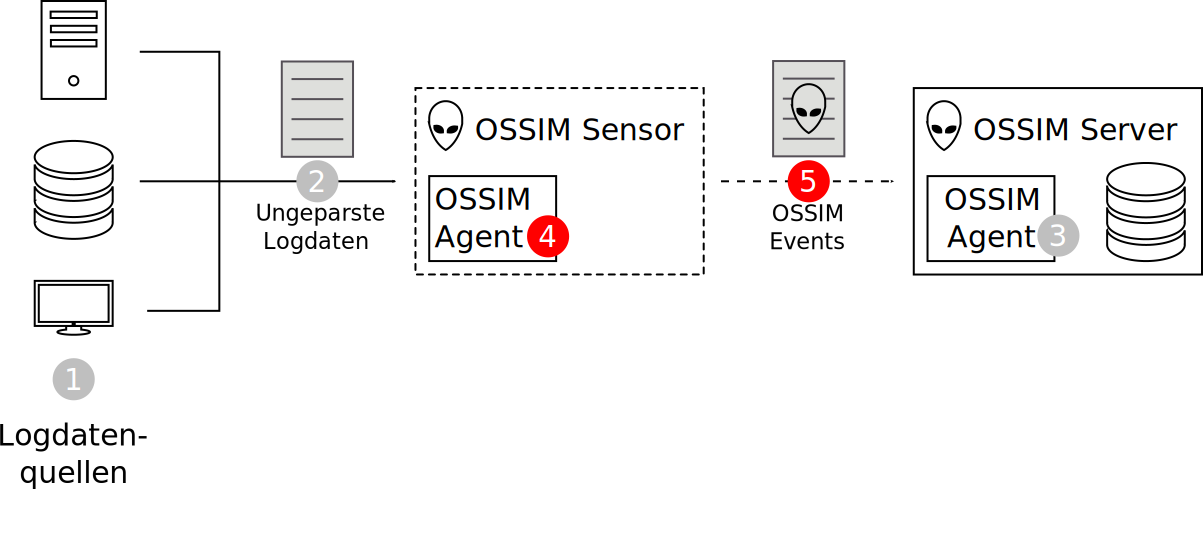
\includegraphics[width=0.9\textwidth]{dia/ossim_data_access_point.pdf}
    \caption{High-Level-Übersicht über die OSSIM-Architektur und den Datenfluss.}
    \label{fig:ossim_data_access_point}
\end{figure}

\begin{enumerate}

\item \textbf{In der Quelle der Logdaten}\\
  Bei diesem Ansatz werden die Daten bereits pseudonymisiert, bevor sie die Datenquelle verlassen. Auch wenn dieser Ansatz aus datenschutztechnischer Sicht die beste Möglichkeit darstellen würde, so ist er doch nicht umsetzbar, da hierzu jede mögliche Quelle von Logdaten universell verändert werden müsste.

\item \textbf{Syslog-Proxy}\\
  Dieser Ansatz pseudonymisiert die Daten vor dem ersten Kontakt mit einer OSSIM-Komponente, indem Datenquellen ihre Logdaten an einen Proxy senden, der die Daten pseudonymisiert und erst anschließend an OSSIM weiterreicht. Hierdurch wird erreicht, dass die Daten zu keiner Zeit nicht-pseudonymisiert in OSSIM vorliegen. Ein Nachteil dieser Lösung ist, dass sie das Parsen und Neuzusammensetzen der Logdaten im Proxy erfordert. \todo{Beschreibung erweitern - analog zu Plugins in OSSIM}

\item \textbf{Patchen des OSSIM-Sensor-Agents}\\
  Bei dieser Lösung müsste der OSSIM-Agent des Sensors so verändert werden, dass vor dem Senden der Events an den Server die Pseudonymisierung stattfindet. Daten erreichen den OSSIM-Server nur pseudonymisiert und mehrfaches Parsen wie in der zweiten Lösung wird verhindert. Auf der anderen Seite erfordert diese Lösung einen Eingriff in die Funktionsweise von OSSIM, was beispielsweise bei Updates von OSSIM zu Problemen führen kann. Außerdem liegen die Daten zu Beginn in nicht-pseudonymisierter Form im Sensor vor. \todo{Syslog-Problematik erwähnen} Zusätzlich erfordert diese Lösung die verteilte Installation von OSSIM-Sensor und -Server, schließt also die Ein-Maschinen-Installation aus \todo{Wording anpassen}.
  
\item \textbf{Sensor-Server-Proxy}\\
  Hier wird ein Proxy zwischen Sensor und Server geschaltet, der bereits geparste Events pseudonymisiert und anschließend an den Server sendet. Dieser Ansatz würde mehrfaches Parsen verhindern und dafür sorgen, dass nur pseudonymisierte Logdaten den OSSIM-Server erreichen. Wie die vorhergehende Lösung würde er jedoch nur in der verteilten Installation funktionieren \todo{Wording} und zusätzlich in die Kommunikation zwischen Sensor und Server aktiv eingreifen, was im Hinblick auf die Nachrichtenintegrität\footnote{
    In der aktuellen Version von OSSIM werden Nachrichten unverschlüsselt und nicht signiert zwischen Sensor und Server versendet, aber zu hoffen ist, dass dieser Zustand sich in zukünftigen Versionen noch ändert.
  } und auch auf geändertes Verhalten nach Updates von OSSIM einen Nachteil darstellt.
  
\item \textbf{Patchen des OSSIM-Servers}\\
  Die letzte Möglichkeit ist das Verändern des OSSIM-Servers selbst. Diese Lösung ist vergleichbar mit der dritten Möglichkeit. Zusätzlich würde sie bei der verteilten sowie bei der Ein-Maschinen-Installation \todo{Wording} funktionieren, auf der anderen Seite aber zulassen, dass nicht-pseudonymisierte Events sogar noch direkt auf dem Server vorliegen.

\end{enumerate}

Insbesondere der aus dentenschutztechnischer Sicht relevante Vorteil, dass die Daten bereits pseudonymisiert in allen OSSIM-Komponenten eintreffen, ließ die Entscheidung auf die zweite Möglichkeit fallen. Dass die Lösung außerdem noch für beide Varianten der OSSIM-Installation möglich ist und keine Anpassungen an OSSIM selbst benötigt, wiegt den Nachteil des zusätzlichen Parsens und wieder Zusammensetzens der Lognachricht bei Weitem auf.\todo{Auch auf Angreifermodell beziehen}


\subsection*{Anforderungen um Bezug auf den Einsatz eines kryptographischen Schwellwertschemas}

- Verteiltes Modell 
- Kommunikation
- ...


\subsection*{Erweiterbarkeit um neue Datenquellen}

- Erweiterbar für neue Datenquellen

\subsection*{Erweiterbarkeit um neue Datenschutztechniken}

Neben der im Fokus dieser Arbeit stehenden Pseudonymisierung und dem Einsatz von kryptographischen Schwellwertschemata zum Schutz der Logdaten gibt es weitere Datenschutztechniken, die für den Anwendungsfall genutzt werden könnten (siehe Kapitel \ref{cha_alternatives}). Der umgesetzte Prototyp sollte leicht um diese Techniken erweiterbar sein.

\todo{Resultate}


\section{Entwurf}

\label{sec_impl_architecture}

\todo{Einführender Absatz}

\subsection{Eingriff in den OSSIM-Datenfluss}

\todo{Hier oder in Anforderungen?}

Für den Eingriff zur Pseudonymisierung der Logdaten bieten sich verschiedene Stellen im Datenfluss von OSSIM an. In diesem Abschnitt sollen die verschiedenen Möglichkeiten dargestellt und gegeneinander abgewogen werden. Eine Übersicht über die verschiedenen Stellen bietet Abbildung \ref{fig:ossim_data_access_point}. Im Folgenden sollen die verschiedenen Möglichkeiten bezogen auf die in Abschnitt \ref{subsec_impl_requirements_ossimintegration} dargestellten Eigenschaften bewertet werden.

\begin{enumerate}

\item \textbf{In der Quelle der Logdaten}\\
  Bei diesem Ansatz werden die Daten bereits pseudonymisiert, bevor sie die Datenquelle verlassen. Auch wenn dieser Ansatz aus datenschutztechnischer Sicht die beste Möglichkeit darstellen würde, so ist er doch nicht umsetzbar, da hierzu jede mögliche Quelle von Logdaten universell verändert werden müsste.

\item \textbf{Syslog-Proxy}\\
  Dieser Ansatz pseudonymisiert die Daten vor dem ersten Kontakt mit einer OSSIM-Komponente, indem Datenquellen ihre Logdaten an einen Proxy senden, der die Daten pseudonymisiert und erst anschließend an OSSIM weiterreicht. Hierdurch wird erreicht, dass die Daten zu keiner Zeit nicht-pseudonymisiert in OSSIM vorliegen. Ein Nachteil dieser Lösung ist, dass sie das Parsen und Neuzusammensetzen der Logdaten im Proxy erfordert. \todo{Beschreibung erweitern - analog zu Plugins in OSSIM}

\item \textbf{Patchen des OSSIM-Sensor-Agents}\\
  Bei dieser Lösung müsste der OSSIM-Agent des Sensors so verändert werden, dass vor dem Senden der Events an den Server die Pseudonymisierung stattfindet. Daten erreichen den OSSIM-Server nur pseudonymisiert und mehrfaches Parsen wie in der zweiten Lösung wird verhindert. Auf der anderen Seite erfordert diese Lösung einen Eingriff in die Funktionsweise von OSSIM, was beispielsweise bei Updates von OSSIM zu Problemen führen kann. Außerdem liegen die Daten zu Beginn in nicht-pseudonymisierter Form im Sensor vor. \todo{Syslog-Problematik erwähnen} Zusätzlich erfordert diese Lösung die verteilte Installation von OSSIM-Sensor und -Server, schließt also die All-In-One-Installation aus.
  
\item \textbf{Sensor-Server-Proxy}\\
  Hier wird ein Proxy zwischen Sensor und Server geschaltet, der bereits geparste Events pseudonymisiert und anschließend an den Server sendet. Dieser Ansatz würde mehrfaches Parsen verhindern und dafür sorgen, dass nur pseudonymisierte Logdaten den OSSIM-Server erreichen. Wie die vorhergehende Lösung würde er jedoch nur in der verteilten Installation funktionieren und zusätzlich in die Kommunikation zwischen Sensor und Server aktiv eingreifen, was im Hinblick auf die Nachrichtenintegrität\footnote{
    In der aktuellen Version von OSSIM werden Nachrichten unverschlüsselt und nicht signiert zwischen Sensor und Server versendet, aber zu hoffen ist, dass dieser Zustand sich in zukünftigen Versionen noch ändert.
  } und auch auf geändertes Verhalten nach Updates von OSSIM einen Nachteil darstellt.
  
\item \textbf{Patchen des OSSIM-Servers}\\
  Die letzte Möglichkeit ist das Verändern des OSSIM-Servers selbst. Diese Lösung ist vergleichbar mit der dritten Möglichkeit. Zusätzlich würde sie bei der verteilten sowie bei der All-In-One-Installation funktionieren, auf der anderen Seite aber zulassen, dass nicht-pseudonymisierte Events sogar noch direkt auf dem Server vorliegen.

\end{enumerate}

\begin{figure}[]
    \centering
        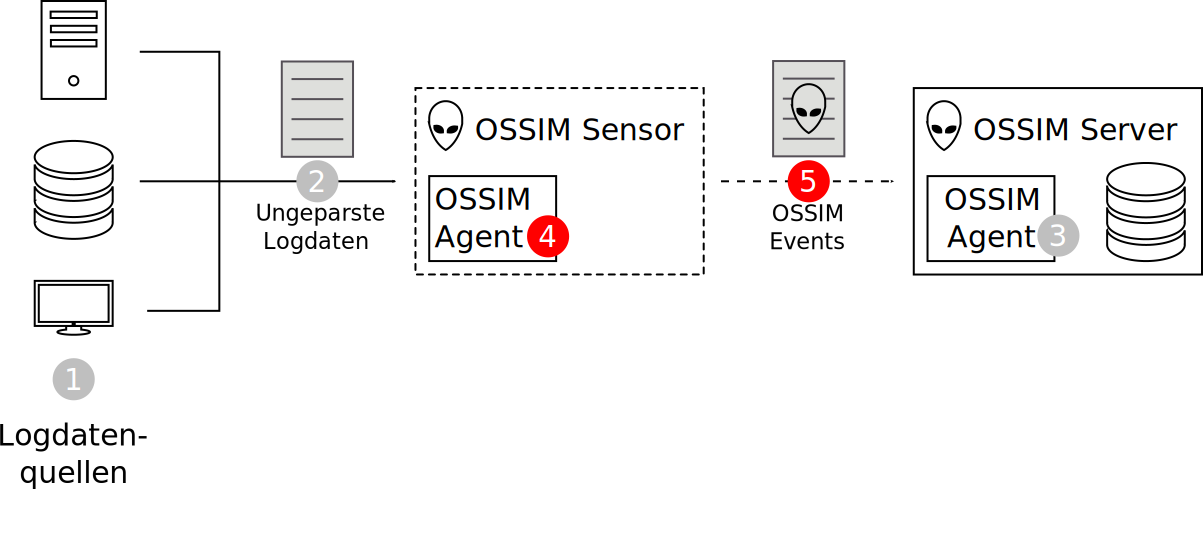
\includegraphics[width=0.9\textwidth]{dia/ossim_data_access_point.pdf}
    \caption{Mögliche Eingriffspunkte in den OSSIM-Datenfluss.}
    \label{fig:ossim_data_access_point}
\end{figure}

Insbesondere der aus datenschutztechnischer Sicht relevante Vorteil, dass die Daten bereits pseudonymisiert in allen OSSIM-Komponenten eintreffen, ließ die Entscheidung auf die \textbf{zweite Möglichkeit} fallen. \todo{Digitalgipfel:   Die	 Pseudonymisierung	 ist	 im	 Verarbeitungsprozess	so	früh	wie möglich	durchzuführen.	 }
Dass die Lösung außerdem noch für beide Varianten der OSSIM-Installation möglich ist und keine Anpassungen an OSSIM selbst benötigt, wiegt den Nachteil des zusätzlichen Parsens und wieder Zusammensetzens der Lognachricht bei Weitem auf.\todo{Auch auf Angreifermodell beziehen}



\subsection{Architektur}

%- Beschreibung Architektur
%
%- Wie deckt dieser Ansatz die Anforderungen ab?
%  - Einbindung OSSIM
%  - Pseudonymisierung
%  - Schwellwert
%  - Benutzerinteraktion
%  - Erweiterbarkeit Datenquellen
%  - Erweiterbarkeit Datenschutztechniken

Ausgehend von diesen Überlegungen wurde ein verteiltes System entworfen, dass die Anforderungen aus Abschnitt \ref{sec_impl_requirements} erfüllt und an der beschriebenen Stelle in den Datenfluss eingreift. 
Einen Überblick bietet Abbildung \ref{fig:high__level_architecture}. Das System besteht aus verschiedenen Komponenten, die im Folgenden näher beschrieben werden.

\begin{figure}[]
    \centering
        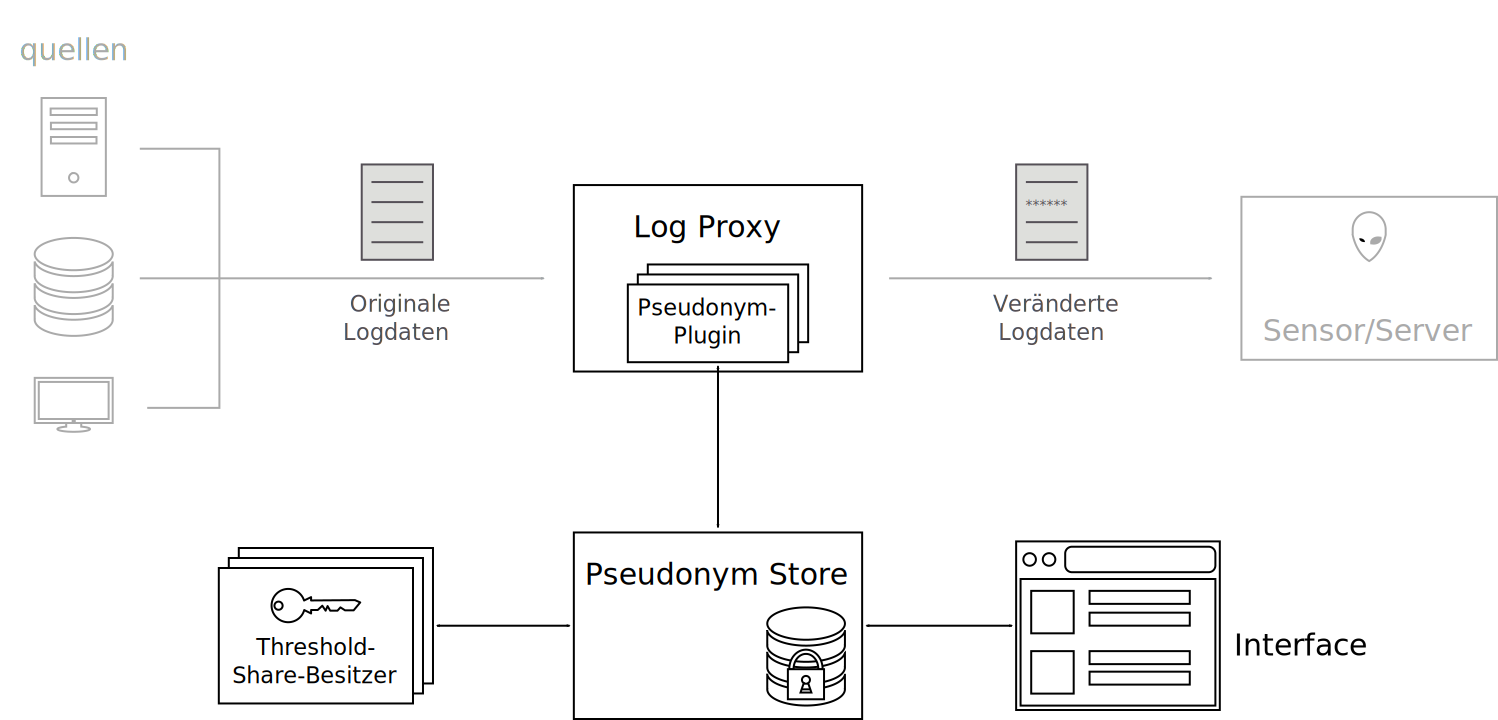
\includegraphics[width=0.9\textwidth]{dia/high_level_architecture.pdf}
    \caption{Ein Überblick über die entworfene Architektur.}
    \label{fig:high__level_architecture}
\end{figure}

Ein \textbf{Log-Proxy}, der die Daten über das Syslog-Protokoll entgegennimmt, verändert und anschließend an OSSIM weiterleitet. Das Verändern der Daten kann mit verschiedenen Plugins geschehen, so dass neben der umzusetzenden Pseudonymisierung auch weitere Datenschutztechniken eingesetzt werden können, was die geforderte Erweiterbarkeit aus Abschnitt \ref{subsec_impl_requirements_plugins} ermöglicht. Der Proxy leistet die Behandlung von Logdaten aus verschiedenen Quellen (siehe Abschnitt \ref{subsec_impl_requirements_differentsources}), was wie bereits im vorhergehenden Abschnitt beschrieben durch Parsen und Wiederzusammensetzen der Daten geschehen muss. Die Konfiguration des quellenabhängigen Vorgehens bei der Logdatenverarbeitung erfolgt ebenfalls hier.

Ein in dem Proxy enhaltenes Plugin wird für die Pseudonymisierung von Daten zuständig und kommuniziert dazu mit einer externen Komponente -- dem Pseudonym-Service. Die Kommunikation mit dem Proxy erfolgt über einen Webservice-basierten Ansatz. Das Plugin kann für eingehende Daten ein Pseudonym anfordern und dieses anschließend in den Logdaten verwenden.

Der \textbf{Pseudonym-Service} erfüllt zwei Aufgaben: das Speichern und Verwalten der Pseudonyme sowie die Integrierung des kryptographischen Schwellwertschemas. Initial muss die Schlüsselgenerierung des Schwellwertschemas (bei zentraler Schlüsselgenerierung) oder die Koordinierung der teilnehmenden Benutzer (bei dezentraler Schlüsselgenerierung) durch den Service geleistet werden. 
Es können während des Betriebs neue Pseudonyme angelegt und zusammen mit ihrem durch das Schwellwertschema verschlüsselten Datum abgelegt werden. Sie werden durch geeignete Maßnahmen durchsuchbar gehalten, um für ein Datum überprüfen zu können, ob bereits ein Pseudonym vergeben wurde. 
Über ein Webinterface kann ein berechtiger Benutzer die Aufdeckung eines bestimmten Pseudonyms fordern und den Status seiner Forderung bzw. im Erfolgsfall das aufgedeckte Datum betrachten. Dieses Datum wird durch das Kombinieren der partiellen Entschlüsselungen erhalten, die von den entsprechenden \textit{Share}-Besitzern berechnet werden.

Benutzer, die zuständig für die Bewertung von Anfragen zur Aufdeckung eines Pseudonyms sind, erhalten die Möglichkeit zur Interaktion mit dem System über eine \textbf{Client-Anwendung}, für die der Pseudonym-Service ebenfalls als Webservice agiert. Diese Anwendungen leisten im Falle der dezentralen Schlüsselgenerierung die initiale Generierung, verwalten den \textit{Share} des Benutzers und können nach der Bestätigung des Benutzers zu der Aufdeckung eines Pseudonyms partiell beitragen. 


\section{Einbindung in OSSIM}

\label{sec_impl_integration_into_ossim}

%- Vorgehen
%
%- Nur für Syslog, keine anderen Fomate betrachtet
%
%- Syslog-Nachrichten werden entgegengenommen, geparst und Config-basiert einzelne Datenfelder bearbeitet (basierend auf RegEx)
%
%- Konfigurationsdateien für Datenquellen (leichte Erweiterbarkeit, auch im Bezug auf neue Datenquellen, ...) mit Beispiel
%
%- Plugins (leichte Erweiterbarkeit, ...)

\todo{Proxy-Aufbau und Vorgehensweise erläutern, insgesamt Abschnitte besser verknüpfen}


Für die in dieser Arbeit zu leistende prototypische Umsetzung des Systems wurde sich auf den am häufigsten\footnote{
  Die in OSSIM bereits mitgelieferten Plugins bestätigen dies. Unter den Hunderten Plugins ist nur ein einziges, das einen anderen Mechanismus als das Syslog-Protokoll nutzt. Auch wenn beispielsweise Plugins, die eine Datenbankabfrage enthalten, immer dem Anwendungsfall angepasst und daher nicht in OSSIM inkludiert werden können, so unterstützt dies doch die Annahme des Syslog-Protokolls als am häufigsten genutzten Weg und damit als geeignet für den Fokus dieser Arbeit.
} genutzten Weg des Datenerhalts in OSSIM (siehe Abschnitt \ref{subsec_state_siem_parsing}) beschränkt: das Entgegennehmen der Daten über das Syslog-Protokoll. 




Die Behandlung von verschiedenen Datenquellen wird durch Konfigurationsdateien ermöglicht:

\begin{lstlisting}[morekeywords={general,active,pattern,group1,group2}]
[general]
active=True

[group1]
pattern=^(?P<time>\w+ *\d{1,2} \d{2}:\d{2}:\d{2}) (?P<device>[^:]+): Testing my device USER=(?P<user>.+)$
time=Substitute(substitute = 'somevalue_time')
device=Substitute(substitute = 'somevalue_device')
user=Pseudonymize()

[group2]
pattern=^(?P<test>.*)$
test=Pseudonymize()
\end{lstlisting}

Eine Konfigurationsdatei kann aus mehreren Bereichen bestehen. Der \texttt{general}-Bereich enthält allgemeine Angaben über das Plugin. Um unterschiedliche Lognachrichten eines Gerätes bündeln zu können, kann eine Konfigurationsdatei weiterhin mehrere Bereiche enthalten, die jeweils die Verarbeitung einer bestimmten Lognachricht beschreiben. Angegeben werden muss jeweils ein regulärer Audruck, der die Nachricht beschreibt und mehrere Gruppen (\texttt{(?P<name>...)}) enthalten kann. Für jede dieser Gruppen muss eine Angabe zu dem Plugin inklusive notwendiger Parameter gemacht werden, dass die Gruppe verarbeiten soll. Durch diese Konfigurationsdateien können Nachrichten unbekannter Formate aus neuen Datenquellen leicht in das bestehende System eingebunden werden.



Die Erweiterbarkeit um neue Datenschutztechniken wird durch leicht erweiterbare Plugins ermöglicht. Ein Plugin muss lediglich die Methode \texttt{handle\_data} implementieren, die die originalen Daten und alle in der Konfiguration angegebenen Parameter erhält. Ein einfaches Plugin, das die Daten durch ein in der Konfiguration angegebenen Wert ersetzt, könnte so aussehen:

\begin{lstlisting}[language=Python]
class Substitute(AbstractPlugin):

    def handle_data(self, data: str, **kwargs) -> str:
        if 'substitute' in kwargs:
            return kwargs['substitute']
        else:
            raise MissingSubstituteError
\end{lstlisting}

\section{Umsetzung der Pseudonymisierung} % und Searchable Encryption

\label{sec_impl_pseudonymity}

% Pseudonymgenerierung

% Parameter: Zeitabhängig, Häufigkeitsabhängig, USE_PFP
% Wie erfolgt die Konfiguration? Wo werden Werte gesetzt/gespeichert?

% MAC Generierung (bzw. Empfang als Search_token) beschreiben

% Zweiter MAC?
% Auch auf Vertrauensmodell im Zusammenhang mit PFP eingehen: Was erfährt die DB, was lässt sich verketten, was würde bei Aufdecken eines Pseudonyms geschehen? Was passiert bei unerlaubtem Zugriff auf gespeicherte Daten?


Für die Pseudonymisierung wurde ein Plugin für den Proxy entwickelt. Bei jedem eintreffenden Logdatum kann abhängig von dem Datenformat für ein entsprechendes Datenfeld ein Pseudonym als Ersatz für das echte Datum gesetzt werden. Dazu stellt der Pseudonym-Service eine Schnittstelle bereit, über die für ein Datum ein Pseudonym erhalten werden kann. Durch diese Trennung wird eine höhere Sicherheit der Zuordnung zwischen Datum und Pseudonym erreicht: In dem Proxy kommen die Logdaten in unveränderter Form an und werden verändert weitergesendet, daher ist die Zuordnung hier implizit bekannt und muss in Kauf genommen werden. Die Speicherung dieser Zuordnung erfolgt jedoch nur in dem Pseudonym-Service. Durch die Verschlüsselung und die in den folgenden Abschnitten beschriebene MAC-abhängige Pseudonymgenerierung erfährt der Pseudonym-Service nichts über das Datum, das durch das Pseudonym beschrieben wird. So führt unberechtigter Zugriff auf die Datenbank des Pseudonym-Service nicht zu mehr Informationen über das Datum, das ein Pseudonym bescchreibt.

Auf der Proxy-Seite wird das verschlüsselte Datum (siehe dazu Abschnitt \ref{sec_impl_threshold}) zusammen mit einem generierten MAC, der wie in Abschnitt \ref{sec_state_se} beschrieben für die Überprüfung auf bereits bestehende Pseudonyme genutzt wird, an den Pseudonym-Service gesendet. 
Der Schlüssel, der für die Generierung des MACs verwendet wird, wird immer nach einer bestimmten Zeitspanne neu generiert. Diese Zeitspanne kann mittels eines Parameters an das Anwendungsszenario angepasst werden (vgl. \ref{sec_state_pseudonymity}). Durch diesen Schlüsselwechsel wird erreicht, das für gleiche Daten, für die der MAC mit einem neuen Schlüssel erstellt wird, auch neue Pseudonyme erhalten werden. \\
Da der Schlüsselwechsel nicht Pseudonym-abhängig geschieht, ist die Zeitspanne global für alle Pseudonyme gültig und somit als maximale Zeitspanne zu verstehen. Dies kann für die Anomalieerkennung evtl. Probleme bereiten, wenn nicht genügend lange Überwachungsdaten verkettet werden können. Auf der anderen Seite würde eine Verweildauer für einzelne Pseudonyme ein Erfassen des Erstellungszeitpunkts in der Datenbank erfordern, was wie in Abschnitt \ref{sec_state_pseudonymity} beschrieben Rückschlüsse auf das ursprüngliche Datum des Pseudonyms liefern könnte. Daher wurde sich gegen diesen Ansatz entschieden.

Auf der Service-Seite wird nun anhand des empfangenen MACs durch Vergleich mit in der Datenbank vorliegenden MACs überprüft, ob bereits ein Pseudonym für das Datum vergeben wurde, das noch nicht zu häufig verwendet wurde. Ist dies noch nicht der Fall, so wird ein noch nicht verwendetes, zufälliges Pseudonym erstellt und zusammen mit dem MAC in der Datenbank gespeichert. Anderenfalls wird das bereits vergebene Pseudonym zurückgeliefert. Die maximale Anzahl an Nutzungen kann analog zur maximalen Zeitspanne ebenfalls mittels eines Parameter gesetzt werden. 

Im Zusammenspiel dieser Parameter kann jedoch noch ein Problem entstehen. Für neu vergebene Pseudonyme, die innerhalb eines Zeitabschnitts durch Überschreiten der maximalen Nutzungsanzahl entstanden sind, liegen in der Datenbank Einträge mit gleichem MAC vor. So wird die Verknüpfung verschiedener Pseudonyme ermöglicht, wenn jemand (berechtigt oder unberechtigt) Zugriff auf die Daten erhält. Das Aufdecken eines Pseudonyms deckt auch alle anderen in diesem Zeitintervall erstellten Pseudonyme implizit auf, was dem in Abschnitt \ref{sec_state_pseudonymity} beschriebenen Prinzip der \textit{Perfect Forward Privacy} widerspricht. 
Dieses Problem kann durch eine zusätzliche MAC-Berechnung auf der Service-Seite verhindert werden, die zusätzlich noch einen Pseudonym-abhängigen Zufallswert einbeziehen muss. Der hierzu verwendete Schlüssel muss dann ebenfalls abhängig von dem bereits beschriebenen Parameter neu generiert werden. Hierdurch enthalten Datenbankeinträge, die innerhalb eines Zeitintervalls zu dem gleichen Datum gehören, durch den einfließenden Zufallswert trotzdem unterschiedliche MACs und die Verkettbarkeit verschiedener Pseudonyme ist verhindert. Jedoch erfordert dieser Ansatz eine MAC-Berechnung pro Datenbankeintrag für jede Anfrage und ist daher aus Performance-Sicht kritisch zu betrachten. Daher wird diese Möglichkeit nicht implementiert. Das bestehende Problem ist jedoch für ein konkretes Anwendungsszenario und bei der Wahl der Parameter -- insbesondere des Zeitintervalls -- zu beachten.


\section{Implementierung und Integration des Schwellwertschemas}

\label{sec_impl_threshold}

Something

\subsection{ThresholdCrypto \glqq Lib\grqq{}}

- Bibliothek, die statuslos in allen Teilen des Systems verwendet werden kann.

- Interface

  \subsubsection{Parametergenerierung}
  
  - Verwendete Gruppen und Auswirkungen fester Parameter? HoC, ...
  
  \subsubsection{Hybride Kryptographie}
  
  - Erzeugung symmetrischer Schlüssel und symmetrische Kryptographie per NaCl(pynacl) -> Authenticated Encryption ChaCha Salsa
  
  - lediglich Verschlüsselung dieses Schlüssels mit dem Schwellwertschema
  
  - von erfahrenen Kryptographen entwickelt
  - getestet
  - schnell
  - Beliebiger Nachrichteninhalt ohne Auswirkungen auf die Verschlüsselung

\subsection{Setup-Verfahren}

auf bereits in impl-pseudonymity geschriebenes zurückgreifen

\subsection{Client-Anwendung}

- Shares empfangen und verschlüsselt abspeichern

- Enthält Webserver um Shares niemals auf dem Server speichern zu müssen

\subsection{Proxy}

- Empfängt PublicKey vom Service und nutzt ihn zur Nachrichtenverschlüsselung




\section{Evaluation}

\label{sec_impl_evaluation}

\subsection{Erfüllung der Anforderungen}

\begin{itemize}
  \item Geeignete Stelle zum Eingriff in den Datenfluss zwischen Logdatenquelle und SIEM-System
  \item Parameterabhängige Generierung eindeutiger, aber in gewissem Rahmen verknüpfbarer Pseudonyme
  \item Sicherer, verteilter Einsatz eines anpassbaren kryptographischen Schwellwertschemas -- vorzugsweise mit verteilter Schlüsselgenerierung
  \item Geeignete Benutzerinteraktion mit dem System an notwendigen Stellen
  \item Erweiterbarkeit um unbekannte Datenquellen
  \item Erweiterbarkeit um weitere Datenschutztechniken
\end{itemize}

...

\subsection{Angriffsmöglichkeiten}

- Zentrale Schlüsselgenerierung (Verweis auf state-distributed)

- Krypto nicht von Kryptographen überprüft (Sidechannel, ...)

- Mögliche Schwächen (sowohl Architektur als auch Krypto, Bezug zum Angreifermodell)

- Scheme leakt Nachrichtenlänge als Vielfaches der Blocklänge -> Paddingscheme?

- Reidentification-Problem (siehe auch Lundin 4.3)

\subsection{Performance}

- Zeitmessungen für einzelne Systemfunktionen

- Performance bzw. Auswirkungen der Nutzung (theoretische Rechenlast, Zeit-/Lastmessung, zusätzlicher Speicherbedarf, ...)














